\chapter{Graphical user interface} \label{sec:graphicalInterface}
This chapter describes a graphical user interface created to visualize the power production of the turbines in the decentralized solution. Furthermore, DDS Blockset for Simulink is presented and how it is used to capture and log data from both the centralized and the decentralized solution.

The graphical user interface has been constructed using Matlab, Simulink and DDS Blockset for Simulink.
These tools combined allows the creation of a Simulink model which taps into the communication of the DDS framework.
The data collected via the Simulink models can then be transferred to Matlab for further processing or visualization.

The main objective of the graphical interface is to visualize what messages is currently flowing in the system but almost as important is the ability to collect data for further analysis.
Matlab is a powerful tool for anlysis and having data transferred live from the DDS framework to Matlab allows for both live as well as in depth analysis on datasets collected during experiments.

Currently only the decentralized solution can be visualized and controlled using the graphical interface. Given the scope and focus of this thesis the value added by visualizing the centralised solution would be minimal. Both the decentralized and centralized solutions are able to log data using the Simulink models.

\section{DDS Blockset for Simulink}
RTI has created a Blockset for Simulink allowing a Simulink model to interact with the DDS Participant and other entities in a DDS enabled network.
The blockset consists of a toolbox containing 6 blocks. Common for all blocks except the DDS Time block is that they can be configured with a default or custom Quality of Service (QoS) profile as well as a sample time. The QoS profile must match the QoS profile used in the network which the Simulink model is to interact with. The sample time is related to the Simulink model and specifies the timeinterval between samples.

\begin{figure}[h]
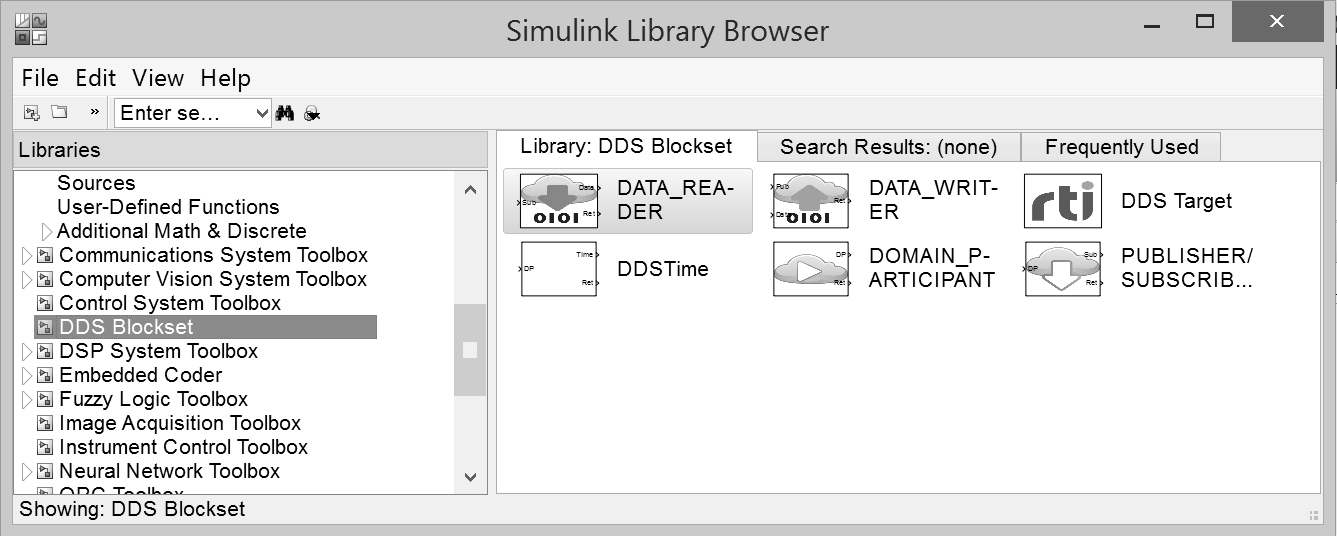
\includegraphics[width=\textwidth]{figures/DDSBlockset}
\captionsetup{format=plain,font=footnotesize,labelfont={bf,defaultCapFont},labelsep=quad,singlelinecheck=no}
	\caption[DDSBlockset blocks for Simulink]{
		\label{fig:DDSBlocksetBlocks} 
		\footnotesize{%
			DDSBlockset blocks for Simulink.
		}
	}
\end{figure}


\paragraph{The DomainParticipant block} is the equivalent to the \textit{DomainParticipant} entity in DDS. This block allows for configuration of a DomainID which links the \textit{DomainParticipant} to a specific DDS domain.

\paragraph{The Publisher/Subscriber block} can be configured as either a \textit{Publisher} or a \textit{Subscriber} and will act as either based on the chosen configuration.

\paragraph{The DataWriter block} is the equivalent to the \textit{DataWriter} entity in DDS. This block can write data to a \textit{Topic} in DDS. The DataWriter block must be configured with the name of the \textit{Topic} as well as the name of the Topic Type created by the Simulink Bus that is input to the DataWriter.

\paragraph{The DataReader block} is the equivalent to the \textit{DataReader} entity in DDS. This block can read data from a \textit{Topic} in DDS. The DataReader block must be configured with the name of the \textit{Topic} as well as the name of the Topic Type created by the Simulink Bus that is input to the DataReader block. The DataReader block can also be configured to either use Read() or Take() for obtaining data from DDS. The Read() command will leave copy data from DDS memory, the Take() command will remove the data from DDS memory. The DataReader block is able to either poll DDS for data, or wait until data is ready or a timeout occurs.

\paragraph{The DDSTarget block} controls how code is generated for the DDS blocks in the Simulink model. It is possible to configure which version of DDS code will be generated for, either RTI Connext DDS(default), or RTI Connext Micro DDS. The type system can be configured to either static or dynamic as well as the discovery mode.

\paragraph{The Time block} returns the current time from DDS output in seconds and nanoseconds.

\section{Simulink model of the centralized solution}\label{subsec:centralizedmodel}
The Simulink model of the centralized solution is presented in \cref{fig:centralizedSimulinkModel}. The centralized solution contains three different messagetypes, TurbineDataMessage, RequestMessage, SetpointMessage, \cref{sec:cenIdl} that all run on different topics. Because of this the centralized Simulink model contains one DomainParticipant, three Subscribers, one for each topic, and three DataReaders, one for each message type, in order to capture the communication in the centralized solution. Every message received is logged to a .mat file together with the current DDS time.

\begin{figure}[!h]
	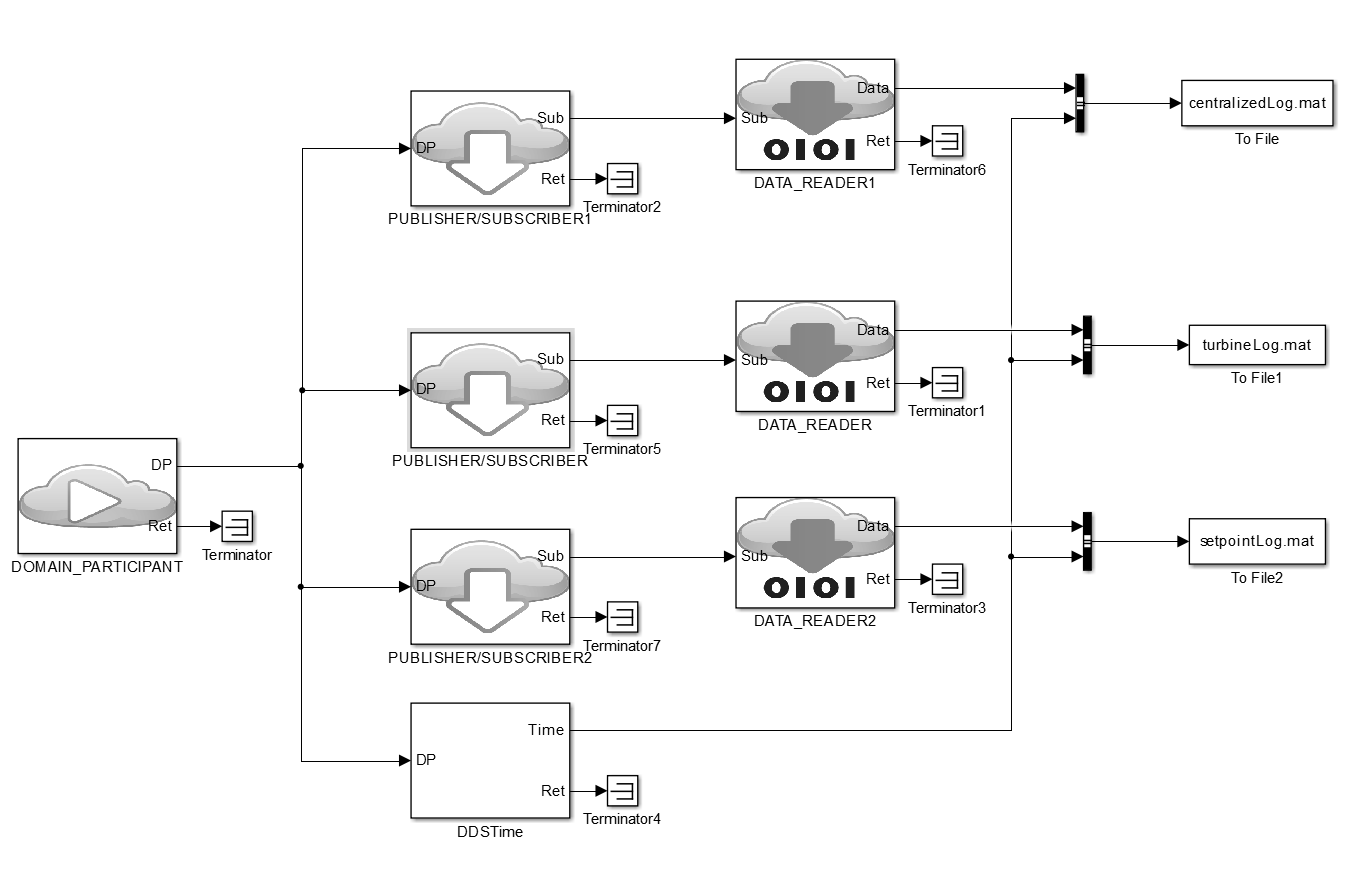
\includegraphics[width=\textwidth]{figures/CentralizedModel}
	\captionsetup{format=plain,font=footnotesize,labelfont={bf,defaultCapFont},labelsep=quad,singlelinecheck=no}
	\caption[Centralized Simulink model]{
		\label{fig:centralizedSimulinkModel} 
		\footnotesize{%
			Centralized Simulink model.
		}
	}
\end{figure}

\section{Simulink model of the decentralized solution}\label{subsec:decentralizedmodel}

\begin{figure}[!h]
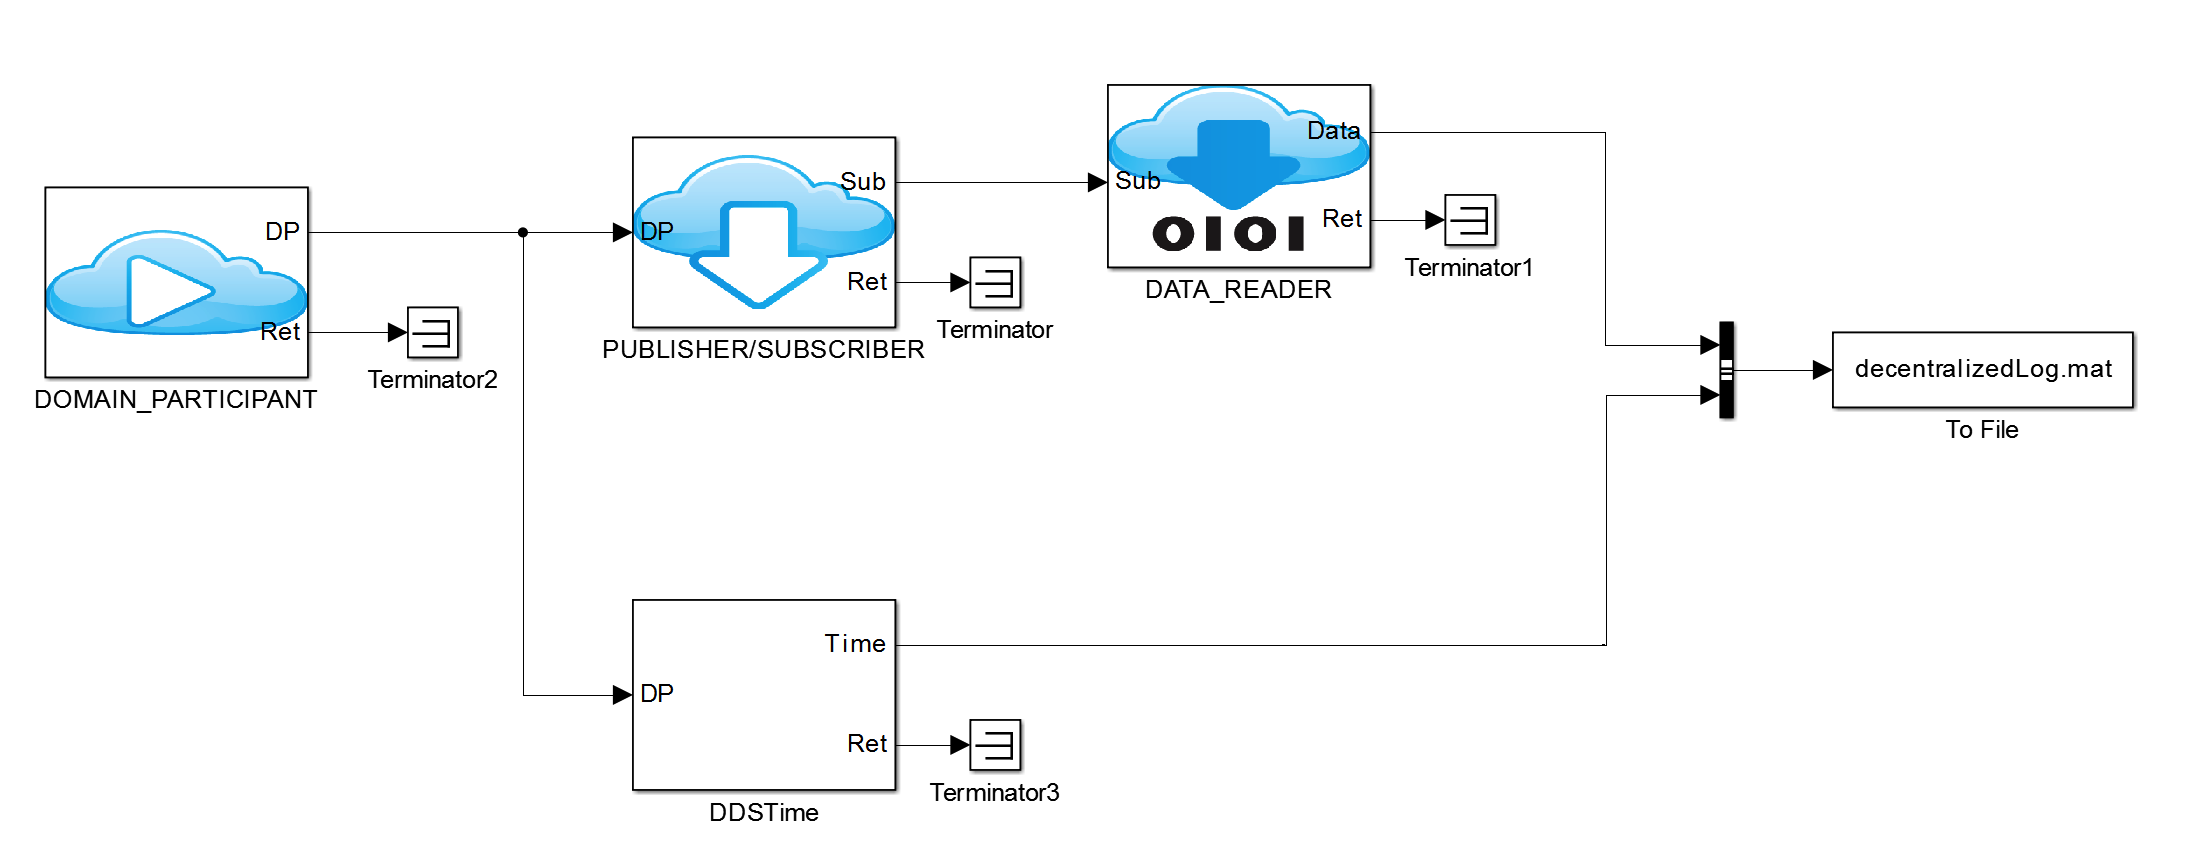
\includegraphics[width=\textwidth]{figures/DecentralizedModel}
\captionsetup{format=plain,font=footnotesize,labelfont={bf,defaultCapFont},labelsep=quad,singlelinecheck=no}
	\caption[Decentralized Simulink model]{
		\label{fig:decentralizedSimulinkModel} 
		\footnotesize{%
			Decentralized Simulink model.
		}
	}
\end{figure}

The Simulink model of the decentralized solution is presented in \cref{decentralizedSimulinkModel}. The decentralized Simulink model has a DomainParticipant block in order to be able to receive data from the same domain as the turbines. It also has a Time block to enable logging and graphing of the current DDS time. Since the decentralized solution only uses one DDS message type, TurbineMessage \cref{sec:decenIdl}, to communicate between the turbines in the system, the decentralized Simulink model has only one Subscriber block and one DataReader block. The Subscriber block specifies the Topic to subscribe to and the DataReader block receives events every time a new TurbineMessage is available. The TurbineMessage that is received is logged to a .mat file together with the current DDS time for later use.

In order to transfer data from the Simulink model to Matlab eventlisteners must be implemented in a Matlab .m file. In the decentralized solution the eventhandler listens for incoming events on the bus object that receives new data from the DataReader block. When new data is received the event fires and data can be collected from the Simulink model. Furthermore, model execution can be controlled from Matlab, as well as parameters like model runtime. 

The eventhandler handling events from the Simulink model appears to be neglecting some of the events published from the Simulink model. This is most likely caused because matlab retains a global shared state that may be overwritten should a new event occur before another event has finished. This results in 'glitches' when drawing the curves for power production on the graphical user interface. The 'glitches' appear in the form of turbines that do not seem to publish new states for several seconds. The reason may be that the eventhandler in matlab ended up as a fairly long function. This combined with the fact that turbine states can be published in bursts may explain why some events are missed.

\section{Installation of DDS Blockset for Simulink}
To install DDS Blockset for Simulink follow the steps provided by Mathworks~\cite{DDSBlocksetPilotSupportPackageUserGuide}. The installation is short but as described below additional work has to be done in order to make DDS Blockset for Simulink work properly with Matlab and Interface Definition Language files.

The problems described in the section all relates to installation of DDS Blockset for Simulink using Matlab 2013b on a Windows 8.1 x64 environment.
Other environments may be more or less optimal but have not been tested during this thesis.

There are a few caveats to be avoided when installing DDS Blockset for Simulink on Windows.
After installation of DDSBlockset for Simulink completes make sure the NDDSHOME path variable is set to \path{C:\Program Files(x86)\RTI}.
Notice that this path is different from the default path recommended by RTI which is \path{C:\Program Files(x86)\RTI\ndds.5.0.0} (version numbers may change).

DDS Blockset for Simulink has an import feature for import of Interface Definition Language files. The import process creates a Simulink bus that the Simulink model can hook into and pull data from. In order to enable import of Interface Definition Language files additional setup must be performed.
Since Matlab does not provide a compiler for C++ on x64 systems one must be downloaded. Microsoft provides a compiler in the Microsoft Windows SDK 7.1. Matlab must be told to use the compiler by using the \path{mex -setup} command. Finally the location of the binaries and the libraries that are downloaded with the new compiler must be added to path.

\section{Evaluation of DDS Blockset for Simulink}
The graphical user interface was mainly created to enable an overview of how the decentralized solution reacts to loss of turbines and changes in the global setpoint for the wind farm. In addition the possibility of logging the data created in both the centralized and the decentralized solutions directly to Matlab for further analysis was compelling.
In retrospective the choice of using DDS Blockset for Simulink may not have been the best available solution. Using DDS Blockset for Simulink as the primary logging tool limited the data available for analysis to the data delivered by the six blocks available in DDS Blockset for Simulink.
Thus, only the data messages delivered by the DataReader block and data delivered by the Time block was useful for further analysis. Additional data about the environment, such as the number of packages sent and received by the machines in the network, is not available through DDS Blockset for Simulink.
Using other tools as for instance the recording and monitoring tools provided by RTI Connext could have proven more efficient in terms of time used for development of the graphical user interface and the Simulink models for capturing and logging data.